\documentclass[10pt,oneside,a4paper]{article}
\usepackage[utf8]{inputenc}
\usepackage{amsmath}
\usepackage{indentfirst}
\usepackage{enumitem}
\usepackage[spanish]{babel}
\usepackage[export]{adjustbox}
\usepackage{graphicx}
\graphicspath{ {img/} }
\usepackage{listings}
\usepackage{subfig}
\usepackage{cite}

\addtolength{\oddsidemargin}{-.300in}
\addtolength{\evensidemargin}{-.300in}
\addtolength{\textwidth}{0.600in}
\addtolength{\topmargin}{-.300in}
\addtolength{\textheight}{0.600in} %1.75

\begin{document}
\begin{titlepage}

\title{\Huge Procesadores Gráficos y Aplicaciones en Tiempo Real  \\[0.7in] \LARGE Mapas de desplazamiento con niveles de detalle\\[3.6in]}
\date{}
\author{Álvaro Muñoz Fernández\\
Iván Velasco González}
\maketitle
\thispagestyle{empty}
\end{titlepage}

\section{Submodulo 1}
\subsection{Primitivas básicas en la etapa de geometría}
El objetivo de esta parte de la práctica consistía en familiarizarnos con la etapa de geometría
dibujando algunas primitivas básicas. Concretamente se debe pintar los vértices que conforman un modelo,
las normales de todos los vértices y por último, superponer el modelo con una representación en modo alambre.

Se puede alternar entre las distintas representaciones mediante la tecla F6, que rotará entre la vista sin añadidos, la visualización de normales, la visualización de alambre y la visualización de vértices.\\

\begin{figure}[h!tbp]
\centering
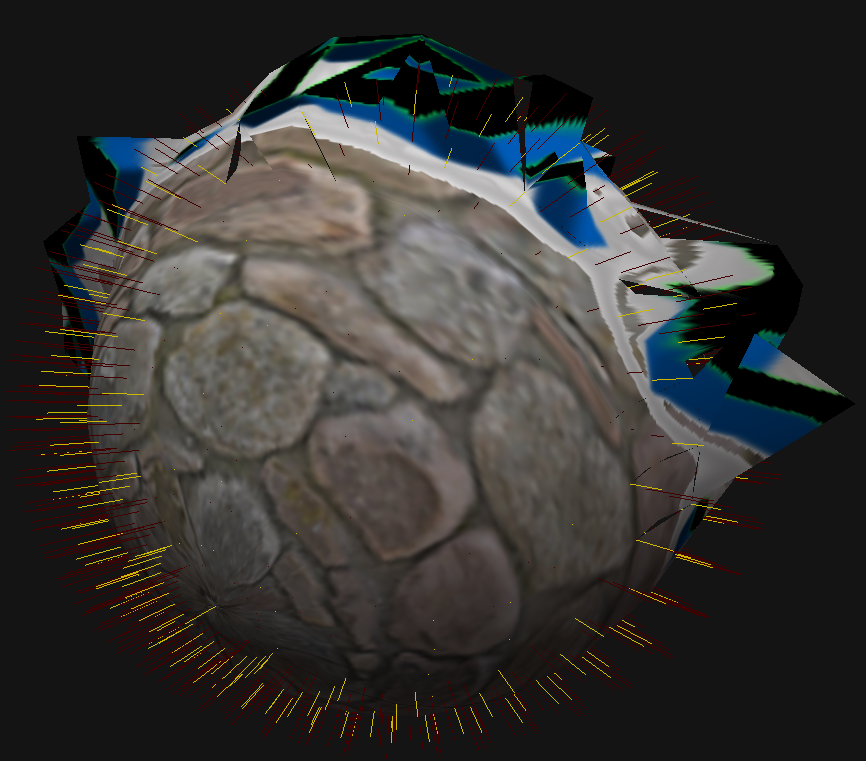
\includegraphics[width=.6\linewidth]{pgatrimgs/Normals.png}
\caption{Representación de las normales del modelo}
\end{figure}

Para la realización de este apartado, lo primero que se ha hecho ha sido añadir a las practicas desarrolladas en G3D(en concreto a la practica de \textit{Deferred Sahing}),
la posibilidad de manejar \textit{shaders} geométricos.\\

En primer lugar, para representar los vértices que conforman un modelo cualquiera se ha programado una etapa de geometría,
la cual tiene como entrada los triángulos del modelo y como salida nuevos vértices que representaran estos vértices del modelo.
Una vez definidos los tipos de entrada y de salida el \textit{shader} solamente debe obtener los vértices que conforman cada triangulo,
desplazarlos ligeramente en la dirección de la normal de cada uno de los vértices (para evitar \textit{Z-fighting}) y pasarlos al \textit{shader} de fragmentos para su procesado.\\

Nótese que para la realización de esta tarea también hubiese sido posible que la entrada del \textit{shader} geométrico hubiesen sido puntos.
Lo cual hubiese ahorrado el procesado de algunos vértices (ya que en el caso de los triángulos están repetidos), pero hubiese sido necesaria otra pasada por el cauce para incorporar este cambio.\\

En segundo lugar, para el dibujado de las normales se ha utilizado la misma entrada que en el caso anterior, es decir, triángulos, pero se ha cambiado la salida a lineas. Ademas ha sido necesario
incluir las normales como una variable de entrada propia que se obtendrá de la salida del \textit{shader} de vértices, y también ha sido necesario incluir una variable de salida que determinará el color de la primitiva.\\

Para crear las lineas que representaran las normales de los vértices, se ha obtenido la posición de cada uno de los vértices que conforman el triangulo y se ha emitido este como un vértice de la linea. El otro vértice ha sido calculado sumándole a este punto inicial la normal multiplicada por un valor de escala, siendo este vértice el final de la primitiva. Además, se ha definido el color de estos vértices como amarillo.\\

Para el caso de la normal del triángulo se han utilizado coordenadas baricéntricas para interpolar tanto la posición como las normales en el punto medio del triángulo. Una vez interpolados estos datos se ha procedido de forma similar que en el caso de los vértices, salvo que en este caso el color que se ha dado a los vértices es rojo.\\

Por último, para el dibujado del modo alambre, se ha realizado un proceso muy similar al realizado para las normales. Siendo la única diferencia que los puntos iniciales y finales de cada primitiva corresponden a los vértices del triángulo, recorriendo por tanto todas las aristas de este. Además, para evitar problemas de \textit{Z-fighting}, es necesario desplazar ligeramente
los vértices emitidos por el \textit{shader} geométrico en dirección a la normal del vértice al que representan.\\

\begin{figure}[htbp]
\centering
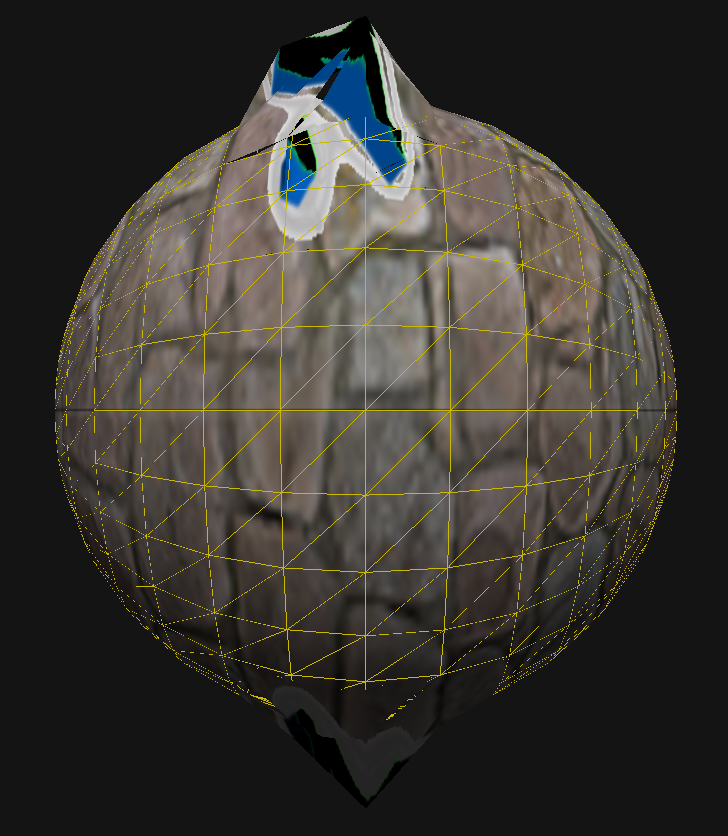
\includegraphics[width=.6\linewidth]{pgatrimgs/WireFrame.png}
\caption{Modo alambre}
\end{figure}


\subsection{\textit{Shader} de teselación}
El objetivo de esta tarea consiste en familiarizarse con el \textit{shader} de teselación para subdividir una geometría dada.
Para ello se ha añadido un \textit{shader} de tipo TCS (\textit{Tessellation Control Shader}), al cual se le pueden especificar los valores de subdivisión por medio de variables \textit{uniform};
y un \textit{shader} de tipo TES (\textit{Tessellation Evaluation Shader}), el cual simplemente calcula la posición del nuevo vértice interpolando con las coordenadas baricentricas proporcionadas como entrada al \textit{shader}.\\

\begin{figure}[!htb]
\centering
    \subfloat[Triángulo]{{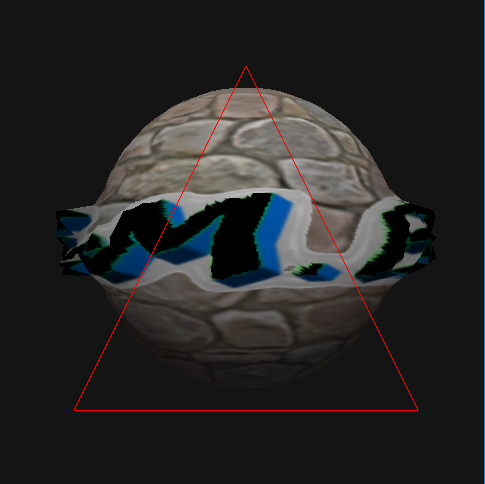
\includegraphics[width=.45\linewidth]{pgatrimgs/geotri.png} }}%
    \qquad
    \subfloat[Quad]{{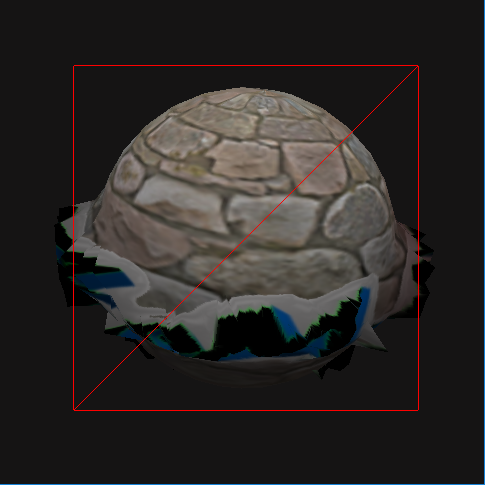
\includegraphics[width=.45\linewidth]{pgatrimgs/geoquad.png} }}%
\caption{Generación de primitivas desde shader de geometría}
\end{figure}

Adicionalmente se han añadido programas que, dado un punto, emplean la etapa de geometría para crear un quad o un triángulo. Utilizando la tecla F7 se activa un overlay que muestra el resultado de estas etapas, rotando entre la generación de un triángulo mediante \textit{shader} geométrica, la generación de un quad, la teselación de un triángulo y la teselación de un quad.\\

\begin{figure}[!htb]
\centering
    \subfloat[Triángulo]{{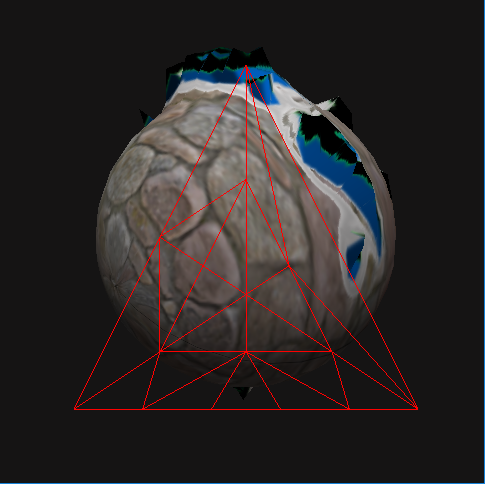
\includegraphics[width=.45\linewidth]{pgatrimgs/tesstri1.png} }}%
    \qquad
    \subfloat[Quad]{{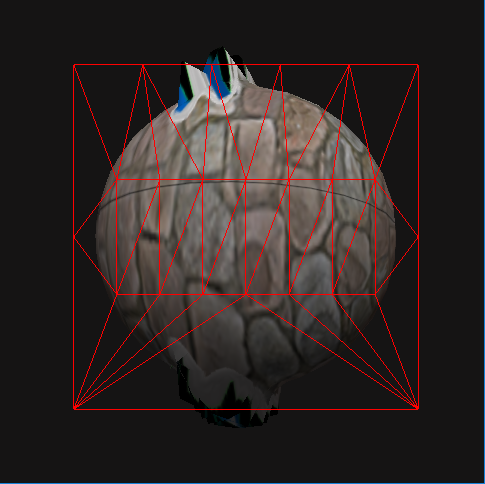
\includegraphics[width=.45\linewidth]{pgatrimgs/tessquad1.png} }}%
\caption{Teselación de primitivas}
\label{fig:tess1}
\end{figure}

Cabe destacar que los \textit{shader} para la teselación del triángulo y del cuadrado son muy similares, cambiando únicamente el numero de puntos que definen un \textit{patch} (4 para el caso del cuadrado y 3 para el caso del triángulo) y rellenando solo los niveles de división interna y externa necesarios para cada caso, aunque con el objetivo de simplificar la interacción se utilizan los mismos valores que los utilizados en el cuadrado. Pueden modificarse estos valores mediante las teclas 'q','w','e','r' para aumentar los niveles de teselación externa, las teclas 'a' y 's' para aumentar los niveles de teselación interna, y las mismas teclas en mayúsculas para disminuir los valores correspondientes.\\

\begin{figure}[!htb]
\centering
    \subfloat[Triángulo]{{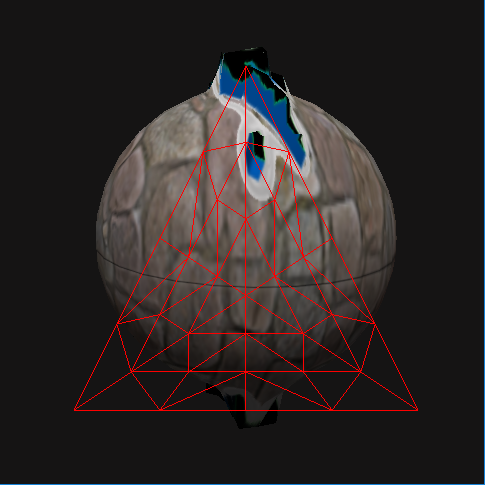
\includegraphics[width=.45\linewidth]{pgatrimgs/tesstri2.png} }}%
    \qquad
    \subfloat[Quad]{{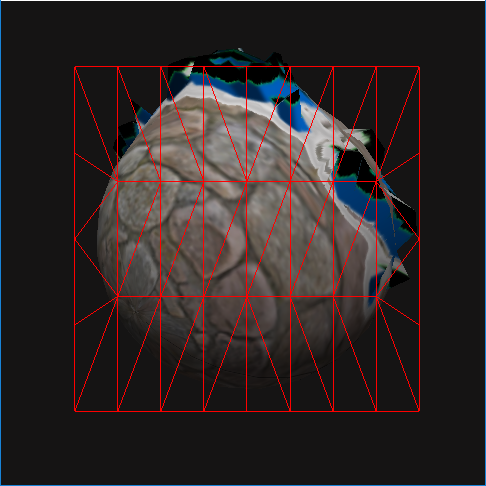
\includegraphics[width=.45\linewidth]{pgatrimgs/tessquad2.png} }}%
\caption{Teselación de primitivas}
\label{fig:tess2}
\end{figure}

Probando con distintas configuraciones de niveles de detalle, hemos llegado a la conclusión que lo que parece mas interesante es mantener unos niveles de teselación interna y externa lo mas parecidos posibles para conseguir un mallado mas regular. Además en el caso del cuadrado parece que los mallados más regulares solamente se consiguen con subdivisiones múltiplo de 2.

Aunque esta son nuestras apreciaciones para el problema enfrentado en esta práctica puede darse el caso de ser útil utilizar niveles de detalle muy dispares. Como en el caso de querer dividir solamente en las aristas del modelo, donde un cuadrado deberá tener gran subdivision en las caras que toquen la arista mientras que no deberá tener ninguna subdivision en la arista contraria para evitar \textit{cracks} con los cuadrados que no se subdividan al no pertenecer a una arista.

En las figuras \ref{fig:tess1} y \ref{fig:tess2} puede apreciarse la diferencia al utilizar distintos valores para la teselación interna y externa.


\section{Submodulo 2}
\subsection{Mapas de desplazamiento}
Este apartado de la practica consiste en la implementación de mapas de desplazamiento con el objetivo de dotar de mayor realismo a la geometría sin tener, por ello, tener que cargar modelos más complejos. Por lo tanto, esta parte de la práctica se divide en dos partes: por un lado en la división de la geometría en la etapa de teselación (también podría hacerse en la de geometría) y por otro lado en el desplazamiento de los vértices en sí, el cual puede realizarse tanto en la etapa de teselación (con el TES) como en el \textit{shader} de geometría. En la figura \ref{fig:disp} puede verse el resultado de aplicar este desplazamiento al elevarse las letras de la textura a partir de una esfera.\\

\begin{figure}[!htb]
\centering
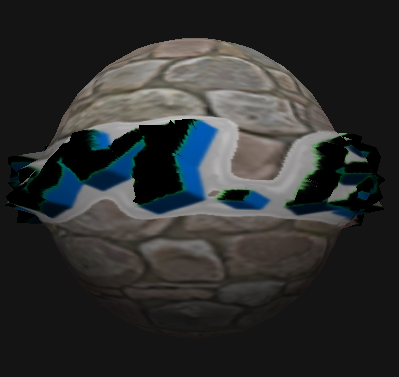
\includegraphics[width=.6\linewidth]{pgatrimgs/Displacement.png}
\caption{Mapa de desplazamiento}
\label{fig:disp}
\end{figure}

En primer lugar, se realiza la subdivisión de la geometría indicando en el TCS unos niveles de teselación fijos (después se verá como se pueden modificar).\\

En segundo lugar se desplazan los vértices para conseguir el desplazamiento, como se ha comentado anteriormente esto puede hacerse tanto en el TES como en el \textit{shader} de geometría.\\

Suponiendo que lo hacemos en el TES el primer paso sería obtener la posición de cada punto generado por el TPG utilizando una interpolación en coordenadas baricéntricas, seguidamente utilizando el mismo método, se obtendrían tanto la normal como las coordenadas de textura de ese nuevo punto.
Una vez tenemos toda esta información procedemos a leer la textura de la que obtendremos el desplazamiento y multiplicaremos el valor leído de la textura (en nuestro caso el canal verde de la textura especular) por la normal obtenida anteriormente para calcular el desplazamiento final que se aplicará al punto, siendo entonces sumado a este.\\

Nótese que para realizar este proceso es necesario definir una seria de variables de entrada que se recibirán del \textit{shader} de vértices como una serie de variables de salida que necesita el \textit{shader} de fragmentos. \\

Ahora, suponiendo que el desplazamiento se realice con el \textit{shader} de geometría el TCS permanece inalterado, ya que no interviene en este proceso, mientras que el TES solamente debe realizar la interpolación de los valores que necesitara en un futuro el \textit{shader} de fragmentos, pero sin desplazar los vértices. Una vez el TES ha pasado todos los datos interpolados al \textit{shader} de geometría, este debe definir la entrada como triángulos (la salida generada por nuestra \textit{shader} de teselación) y la salida como una tira de triángulos que definirá la malla.
Por último, para desplazar los vértices en sí el proceso es completamente igual al caso del TES, simplemente se aplica el desplazamiento a cada uno de los vértices del triangulo y se conforma un nuevo triangulo con el desplazamiento.\\

Como se puede observar en la práctica al cambiar de un modo a otro (tecla F8) rel resultado es exactamente el mismo. Sin embargo, el proceso sería conveniente realizarlo en el \textit{shader} de teselación, ya que siendo el resultado idéntico nos ahorramos una etapa del cauce. 


\subsection{Detalle adaptativo}
En este parte de la practica se propondrá una implementación para variar el nivel de detalle en función de la distancia a la camara. Más concretamente cada triángulo del objeto mostrado se dividirá en mayor o menor medida en función de esta distancia. Por lo tanto, se obtendrán distintos niveles de detalle para un mismo objeto en pantalla.

Para ayudar a la visualización de la geometría se ha añadido una opción de visualización en alambre del modelo que puede activarse y desactivarse con la tecla F9.\\

Para su implementación, en primer lugar se ha decidido que existirán 10 niveles de subdivisión posibles y se le asignara un nivel u otro a cada \textit{patch} (triángulos en nuestro caso, al tratarse de \textit{patches} de 3 vértices) dependiendo de su distancia a la cámara. Por lo tanto nuestro volumen de visualización está dividido en 10 zonas que permiten distintos niveles de detalle.\\

Una vez escogido el nivel de detalle adecuado este se asigna al nivel de teselación interno del triangulo, quedando los niveles de teselación externos fijados a una constante independiente de la distancia con el objetivo de evitar \textit{cracks}, ya que de caso contrario los triángulos de un mismo objeto pueden encontrarse en zonas con distinto nivel de detalle y por tanto,distintos niveles de subdivisión externa.\\

Otra posible implementación que no requiere que los niveles de teselación externos estén fijos para evitar \textit{cracks} hubiese sido la teselación adaptativa de todo el objeto en función de la distancia de este a la cámara, lo cual evita el problema de los \textit{cracks} ya que todos los triángulos del mismo objeto tendrán siempre un nivel de división externo igual. Pero en nuestro entorno en el cual la cámara esta fija esta aproximación carece de sentido, así que se ha aplicado la teselación adaptativa en función de la distancia de cada \textit{patch}.\\

La figura \ref{fig:tesscomp} muestra una comparativa de la geometría generada en el modelo dependiendo de la distancia. En el primer caso puede distinguirse una cantidad de triángulos mucho mayor en la zona de la M, al encontrarse más cerca de la cámara, que en la segunda imagen es mucho más reducida al encontrarse más alejada de la cámara.

\begin{figure}[tbp]
\centering
    \subfloat[Mayor detalle en zona desplazada]{{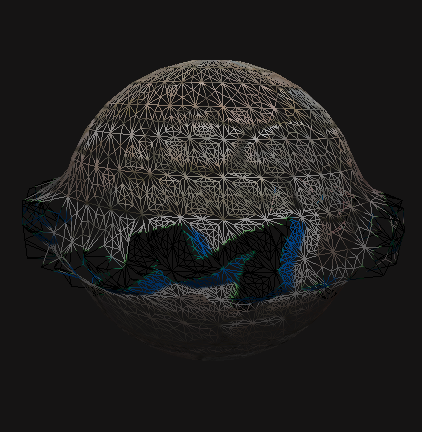
\includegraphics[width=.8\linewidth]{pgatrimgs/LODTessellation1.png} }}%
    \qquad
    \subfloat[Menor detalle en zona desplazada]{{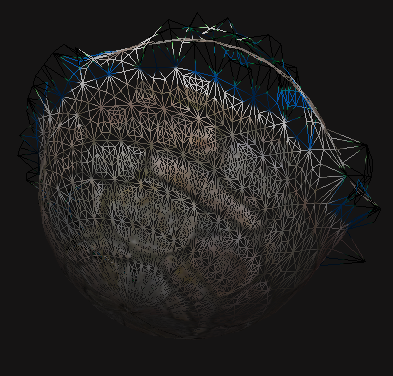
\includegraphics[width=.8\linewidth]{pgatrimgs/LODTessellation2.png} }}%
\caption{LOD-based Tessellation}
\label{fig:tesscomp}
\end{figure}

\end{document}